\documentclass[12pt]{report}

% Essential packages
% \usepackage[french]{babel}
% \usepackage[T1]{fontenc}

\usepackage[margin=2cm]{geometry} % decrease margin
\usepackage{graphicx} % include images
\usepackage{hyperref} % urls, hyperlinks, etc
\usepackage{pdfpages} % include pdf pages
\usepackage{enumitem} % customize itemize
\usepackage[backend=bibtex]{biblatex} % bibliography
\usepackage{csquotes} % Quote bibliography and add hyperlinks
\usepackage{titlesec} % Modify chapter headings
\usepackage{wrapfig} % wrap text around figures
\usepackage{float} % force figure positions at the end of the file
\usepackage[linesnumbered,ruled,vlined]{algorithm2e}
\usepackage{dirtytalk}

\addbibresource{biblio.bib}

% Customize itemize item markers
\renewcommand\labelitemi{-}

% Add source to figures caption
\newcommand*{\captionsource}[2]{%
    \caption[{#1}]{%
        #1%
        \\\hspace{\linewidth}%
	\textbf{Source:} \textit{#2}%
    }%
}

% Some settings for the title page
\titleformat{\chapter}[display]{\normalfont\huge\bfseries}{}{0pt}{\Huge}
\titlespacing*{\chapter} {0pt}{20pt}{40pt}

% Force footnotes to stay on one page
\interfootnotelinepenalty=10000

\begin{document}

\begin{titlepage}
    \newcommand{\HRule}{\rule{\linewidth}{0.5mm}} % Defines a new command for the horizontal lines, change thickness here

    \centering
    \begin{minipage}{.25\textwidth}
	    \centering
	    
\includegraphics[width=80pt]{../imgs/ENSIMAG.png}\\[1cm]
    \end{minipage}%
    \begin{minipage}{.25\textwidth}
	    \centering
	    
\includegraphics[width=80pt]{../imgs/uga-logo.png}\\[1cm]
    \end{minipage}%
    \begin{minipage}{.25\textwidth}
	    \centering
	    
\includegraphics[width=80pt]{../imgs/ryax-logo.png}\\[1cm]
    \end{minipage}%
    \begin{minipage}{.25\textwidth}
	    \centering
	    \includegraphics[width=80pt]{../imgs/logo-LIG.jpg}\\[1cm]
    \end{minipage}

    \vspace{4cm}
    \textsc{\Large End of Studies Master's Project}\\[0.5cm]
    \textsc{\large Master's Thesis}\\[0.5cm]

    \HRule \\[0.4cm]
    { \huge \bfseries Simulation of a Kubernetes Cluster with Validation in Real Conditions}\\[0.4cm]
    \HRule \\[3cm]

    \begin{minipage}{0.4\textwidth}
        \begin{flushleft}
            \large
	    \textit{Author}\\
            Théo \textsc{Larue}
        \end{flushleft}
    \end{minipage}
    ~
    \begin{minipage}{0.4\textwidth}
        \begin{flushright}
            \large
	    \textit{Evaluator}\\
	    Surname \textsc{NAME}
        \end{flushright}
    \end{minipage}

    \vspace{2cm}

    \vspace{2cm}
    \vfill
    \textsc{\large February 24th to August 7th 2020}\\[0.5cm]


\end{titlepage}

\tableofcontents
\newpage

\chapter{Introduction / Abstract}
TODO


\chapter{HPC, Kubernetes and the scheduling problem}

\section{Kubernetes concepts}

In the early stages of application development, organizations used to run their
services on physical servers. With this direct approach came a few
problematics: resources allocation, maintainability, scalability for exemple.
Developers then went on with virtualized machines to run their services
regardless of physical infrasctucture, which then led to the concept of
containers.

\begin{figure}[h]
	\centering
	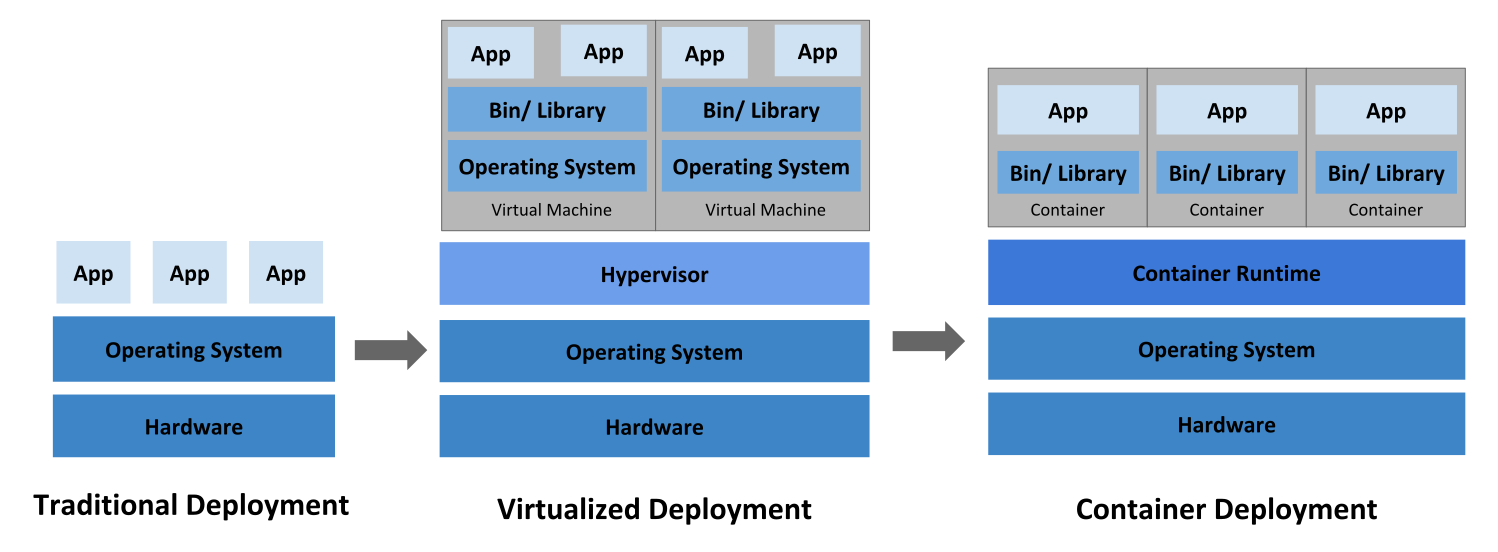
\includegraphics[width=\textwidth]{../imgs/container_evolution.png}
	\captionsource{Evolution of application deployment.}{https://kubernetes.io/docs/concepts/overview/what-is-kubernetes/}
	\label{fig:container-evolution}
\end{figure}

Containers can be thought of as lightweight virtual machines. Unlike virtual
machines, containers share the same kernel with the host machine but still
allow for a very controlled environment to run applications. There are many
benefits to this : separating the development from deployment, portability,
easy resource allocation, breaking large services into smaller micro-services
or support of continuous integration tools (containers greatly facilitate
integration tests), to cite a few.\\

Kubernetes\footnote{\url{https://kubernetes.io/}} aims at automating of the process of deploying,
maintaining and scaling containerized applications. It is an open source
platform originally designed by Google and now maintained and developed by the
Cloud Native Computing Foundation\footnote{\url{https://www.cncf.io/}}. It is
industry grade and widely used by web services, big or small, for its -
relative - ease of use and its reliability.

The basic processing unit of Kubernetes is called a \textbf{pod}. A pod is composed of
one or several containerized applications and volumes (A volume is some storage
space on the host machine that can be linked to containers, so they can read
persistent information or store data in the long term). In the cloud native
context a pod can be thought of as a service or micro-service, but we will see
them a little bit differently.

Pods are bundled together in \textbf{nodes} (figure \ref{fig:node-overview}),
which are most of the time physical machines (but might as well be virtual
machines). They represent another layer to be passed through to access the
outside world which can be useful to add some layers of security or facilitate
communication between pods, for example. Each node runs at least one pod and
also one kubelet which is a process responsible for communicating with the rest
of Kubernetes (or more precisely, with the master node which in turns
communicates with the api server). A set of nodes is called a \textbf{cluster}.
Each Kubernetes instance is responsible for running one cluster.

\begin{figure}[h]
	\centering
	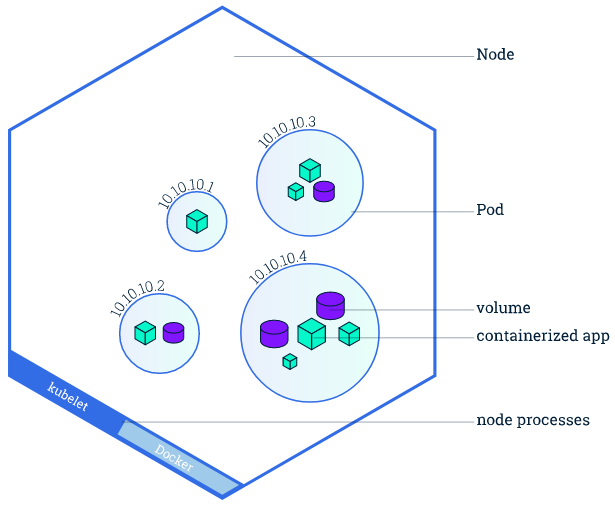
\includegraphics[scale=0.5]{../imgs/node-overview.png}
	\captionsource{Node overview}{https://kubernetes.io/docs/tutorials/kubernetes-basics/explore/explore-intro/}
	\label{fig:node-overview}
\end{figure}


\begin{figure}[]
	\centering
	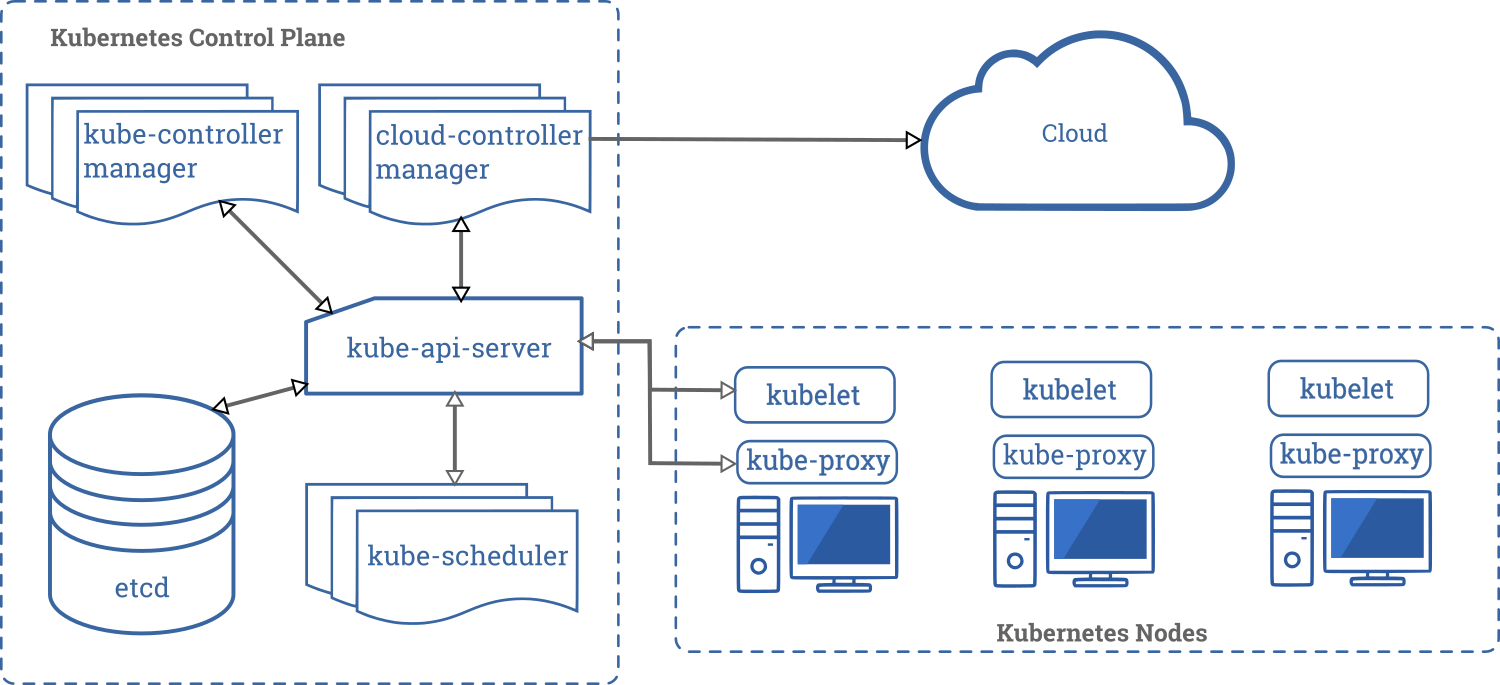
\includegraphics[width=\textwidth]{../imgs/components-of-kubernetes.png}
	\captionsource{Components of Kubernetes}{https://kubernetes.io/docs/concepts/overview/components/}
	\label{fig:kube-components}
\end{figure}

Kubernetes revolves around a central component, its api server (figure
\ref{fig:kube-components}). The majority of every operations go through this
api server : user interactions through kubectl, scheduling operations, saves of
kubernetes state in etcd\ldots We will focus on the lower-right part of this
figure, that is to say the scheduler, the api server and the cluster itself.


\section{HPC and Kubernetes}
A general definition of HPC would be :
\say{\textit{High Performance Computing (HPC) most generally refers to the
		practice of aggregating computing power in a way that delivers
		much higher performance than one could get out of a typical
		desktop computer in order to solve large problems in science,
		engineering, or
		business.}}
\footnote{\url{https://wwwen.uni.lu/university/high_performance_computing}}

HPC can either refer to ``High Performance Computing'' or ``High Performance
Computer'' but it is generally clear which one it refers to, given the
context.
An HPC workload is mostly caracterized by parallel tasks that run on a large
amount of compute units - refered to as ``nodes''.

TODO




\section{The scheduling problem}

\section{Simulating infrastructures}
\subsection{HPC simulators}
\subsection{Kubernetes simulation}

This raises the question of scheduler development. Developing a scheduler
implies being able to test its performances throughout the development process,
however, testing in real conditions is time consuming and expensive.
Organizations can either have enough resources to cover these costs, or test
their scheduler against a simulation.\\

Kubernetes cluster simulations is an open problem and is the subject of this
master project. Our approach relies on the Batsim\cite{batsim} infrastructure
simulator, which is itself built upon Simgrid\cite{simgrid}. Batsim is
currently mostly used to simulate HPC infrastructures but was designed to be
able to simulate any kind of infrastructure and therefore is theoretically able
to simulate any Kubernetes cluster, moreover, Kubernetes was designed to run
services but is capable of handling High-Performance
Computing\cite{kube-for-hpc}. This project aims at adapting Batsim so it can
evaluate Kuberenetes schedulers.

\section{The Batsim infrasctucture simulator}
\subsection{Batsim concepts}

\subsection{Limitations}


\chapter{Problematic}

\section{Objectives}

The goal of this project is to design and implement Batkube, which will be an
interface between Batsim and Kubernetes schedulers. With this interface, we
want to compare Batsim results gainst data from a real Kubernetes cluster,
given HPC workloads.

\section{Translation}

\section{Synchronization}

\chapter{Implementation}

\section{Batkube architecture}
TODO

\section{API implementation}
\section{Time hijack}
TODO

\subsection{batsky-go}
\SetKwInput{KwInput}{Input}
\SetKwInput{KwOutput}{Output}


\begin{algorithm}[H]
\DontPrintSemicolon
\KwInput{req: request channel, res: result channel map}
\While{Batkube is not ready} {
	wait\;
}
requests = []request\;
\While{req is not empty} {
	m = $<$- req \tcc{Non blocking receive}
	requests = append(requests, m)\;
}
sendToBatkube(requests) \tcc{Only requests with duration > 0 are actually sent. Batkube will always anwser.}
now = responseFromBatkube()\;
\For{m in range requests} {
	res[m.id] $<$-now \tcc{The caller continues execution upon reception}
}

	
\caption{Requester loop}
\label{alg:reqLoop}
\end{algorithm}


\begin{algorithm}[H]
\DontPrintSemicolon
\KwResult{Current simulation time}
\KwInput{d: timer duration, req: request channel, res: response channel map}
\KwOutput{now : simulation time}

\If{requester loop is not running}{
	go runRequesterLoop() \tcc{There can on ly be one loop runing at a time}
}
id = newUUID()\;
m = newRequestMessage(d, id) \tcc{Requests are identified using uuids}
resChannel = newChannel()\;
res[id] = resChannel \tcc{A channel is associated with each request}
req $<$- m \tcc{The code blocks here until request is handled}
now = $<$-resChannel \tcc{The code blocks here until response is sent by the requester loop}
return now\;
\caption{Time request (time.now())}
\label{alg:now}
\end{algorithm}



\chapter{Evaluation}

\chapter{Conclusion}


\printbibliography
\end{document}
